\chapter{Практическая часть}

\section{Выбор инструментов}

Для реализации алгоритма были изучены и использованы
следующие инструменты и технологии:

\begin{itemize}
    \item CGAL(The Computational Geometry Algorithms Library) -
    библиотека алгоритмов вычислительной геометрии
    написанная на C ++. Распостраняется под GPL/LGPL лицензией,
    что дает возможность свободно копировать и использовать 
    програмные компоненты.
    Содержит так же полностью комерческие и не доступные для можификации модули.
    В этом проекте таковые не используются.
    \item CMake - кросплатформенная система
    для управления процессом сборки программного обеспечения
    из исходного кода. Является open-source проектом.
    \item Microsoft Visual Studio 2017 - интегрированная среда разработки
    для операционных систем семейства Windows.
    Использовалась под учебной лицензией полученой в
    MSDN(Microsoft Developer Network).
    \item gnuplot - свободная программа для создания двух- и трёхмерных графиков.
    Программа также может генерировать код на LaTeX,
    позволяя использовать шрифты и формулы LaTeX.
    Распостряняется под свободной лицензией.
    \item Git - система контроля версий исходного кода.
    Выпущена под лицензией GNU GPL версии 2
    \item Boost.Python - часть семейства библиотек Boost,
    обеспечивающая возможно прямого взаимодействия между языками С++ и Python. 
    Распостраняется под собственной лицензией Boost Software License.

\end{itemize}

Исходный код всех проектов полученных
в результате научно иследовательской работы находится
в открытом доступе в Git-репозитории на сайте https://github.com/ArchStanton9/polygons


\section{Алгебраическая сумма}

Другое название - <<сумма Минковского>>.

\begin{equation}
    A \oplus B = \{x + y | x \in A, y \in B \}  
\end{equation}


\begin{figure}
    \centering
    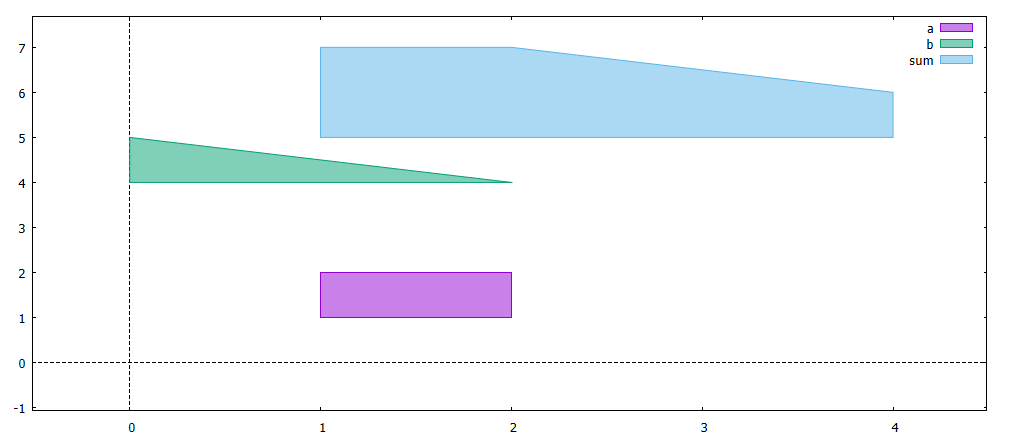
\includegraphics[width=1.0\textwidth]{sum} 
    \caption{Сумма Минковского}
    \label{fig:sum}
\end{figure}
 

Сумма двух выпуклых многоугольников P и Q с m и n вершин
строится довольно просто.
$P \oplus Q$ - выпуклый многоугольник,
ограниченный копиями $m + n$ ребер,
упорядоченных по углу, который они образуют с осью x.
Поскольку два входных многоугольника выпуклые,
их ребра уже отсортированы по углу,
который они образуют с осью x. 
Поэтому сумму Минковского можно вычислить,
используя операцию,
аналогичную шагу слияния в алгоритме <<сортировки слиянием>> за линейное время $O(n+m)$.

В случае невыпуклых многоугольников,
CGAL предлагает два алгоритма:
метод \textit{декомпозиции} и метод \textit{свертки}.

В перовом случае, P и Q разделяются на выпуклые многоугольники.
Получается два набора многоугольников $P_1 \dots P_k$ и $Q_1 \dots Q_l$.
После этого попарно считаются суммы их суммы:

\begin{equation}
    S_{ij}=P_i \oplus Q_j   
\end{equation}

В конце вычисляется объединение полигонов,
и получается итоговая сумма:

\begin{equation}
    P \oplus Q = \bigcup\limits_{i,j} S_{ij}
\end{equation}


Такой подход основан на успешной декомпозиции
входных многоугольников на выпуклые части,
а его производительность зависит от качества разложения.

Для многоуголиников сложной формы,
выгоднее использовать метод свертки.
Пусть P и Q многоугольники с вершинами
$p_0, \dots, p_{m-1}$ и $q_0, \dots, q_{m-1}$
Предположим, что и P, и Q имеют положительные ориентации, т.е
их границы вращаются против часовой стрелки относительно нормали.
Сверткой $P * Q$ называется множество из отрезков $[p_i+q_j, p_{i+1}+q_j]$
состоящее из точек, для которых вектор $\overline{p_i,p_{i+1}}$ 
лежит между $\overline{q_{j−1}q_j}$ и $\overline{q_jq_{j+1}}$,
а так-же по симетрии из $[p_i+q_j, p_i+q_{j+1}]$,
где вектор $\overline{q_i,q_{i+1}}$
лежит между $\overline{p_{i-1},p_i}$ и $\overline{p_i,p_{i+1}}$.

Отрезки свертки образуют множество ломаных кривых,
называемых \textit{циклами свертки}. Сумму $P \oplus Q$ составляют точки,
для которых порядок относительно циклов свертки $P * Q$ не равен нулю.


\section{Геометрическая разность}

Геометрическая разность - операция обратная сумме Минковского:

\begin{equation}
    A \ominus B = \{x: x + B \in A \}
\end{equation}

Эту операцию можно реализовать при помощи алгебраической суммы,
если взять множества А до вмещающего его пространства,
сложить с отражением множества B, 
и дополнение от полученной суммы
будет являться геометрической разностью.
В общем виде это можно записать так:

\begin{equation}
    A \ominus B = (\overline{\overline{A} \oplus - B})
\end{equation}